\documentclass[10pt,landscape]{article}
\usepackage[landscape]{geometry}
\usepackage{multicol}

\usepackage{mathtools}
\usepackage{amsmath}
\usepackage{amsfonts}
\usepackage{xfrac}
\usepackage{graphicx}

% Make the margins tight
\geometry{top=1cm, right=1cm, bottom=1cm, left=1cm}

% remove headers and footers
\pagestyle{empty}

% Make paragraph splits smaller
\setlength{\parindent}{0pt}
\setlength{\parskip}{0.5ex}

% Make the section headings smaller, inspired by the class Latex2e
% quick reference sheet.
\makeatletter
\renewcommand{\section}{\@startsection{section}{1}{0pt}%
                        {-1.3ex}{0.7ex}{\normalfont\large\bfseries}}
\renewcommand{\subsection}{\@startsection{subsection}{2}{0pt}%
                           {-1.3ex}{0.7ex}{\normalfont\normalsize\bfseries}}
\renewcommand{\subsubsection}{\@startsection{subsubsection}{3}{0pt}%
                              {-1.3ex}{0.7ex}{\normalfont\small\bfseries}}
\makeatother

% Remove section numbers
\setcounter{secnumdepth}{0}

% Utility commands
\newcommand{\spto}{\;\to\;}
\newcommand{\spbackslash}{\;\backslash\;}
\newcommand{\nquad}{\!\!\!\!\!\!}
\newcommand{\impl}{\Rightarrow}

\newcommand{\subheading}[1]{\textbf{#1} \vspace{3pt} \\}

% temp length variable
\newlength{\templength}

%% TODO
% Regular Languages
% - DFA formalism
% - Talk about NFA/DFA conversion,
% - NFA/DFA closures even under closures
% - Pumping lemma shortcuts
%   e.g. answer 'how do I reverse an NFA
% - DFA minimization
% - DFA to RE-conversion
%
% Context-Free languages:
% - CFL formalism
% - RL and LL to NFA/DFA conversion
%   - RL conversion via reversal closures
% - Shortcuts for solving pumping lemmas
% - Chompsky Normal form
% - CFG -> PDA conversion 
% 
% Cardinality
% - Schroder-Bernstein theorem
% - Mapping multiple values of the same
% - Cardinality using a paring function.
%
% Turing Machines
% - TM formalism
% - How to make a Turing machine 
% - DTM / NDTMs
% - Turing Machine terminology (acceptance, halting, rejection, deciders)
%
% Undecidability
% - First-principals proof of halting problem
% - Mapping reductions
% - Rice's Theorem
%
% NP-Completeness
% - Definitions of P, NP, NP-complete, and NP-hard.
% - Talk about Turing verifiers (For showing L is in NP)
% - Talk about how to prove a language is NP-complete

\begin{document}
\begin{multicols*}{3}

\begin{center}
    \Large CS3100 Final Note Sheet
\end{center}
\vspace{-0.5cm}

\section{Notation}
\begin{tabular}{rp{0.79\linewidth}}
$L^R$ & The reversal of language $L$. \\
$L^*$ & The Kleene-Star of $L$. \\
$AB$ & The concatenation of language $A$ and $B$. \\
$h(L)$ & A homomorphism (a function that maps every input to 
         a unique output) of $L$. \\
$A \spbackslash B$ & Set difference of $A$ and $B$. $A - B$ is the same thing. \\
\end{tabular}

\section{Chomsky Hierarchy}
\begin{center}
    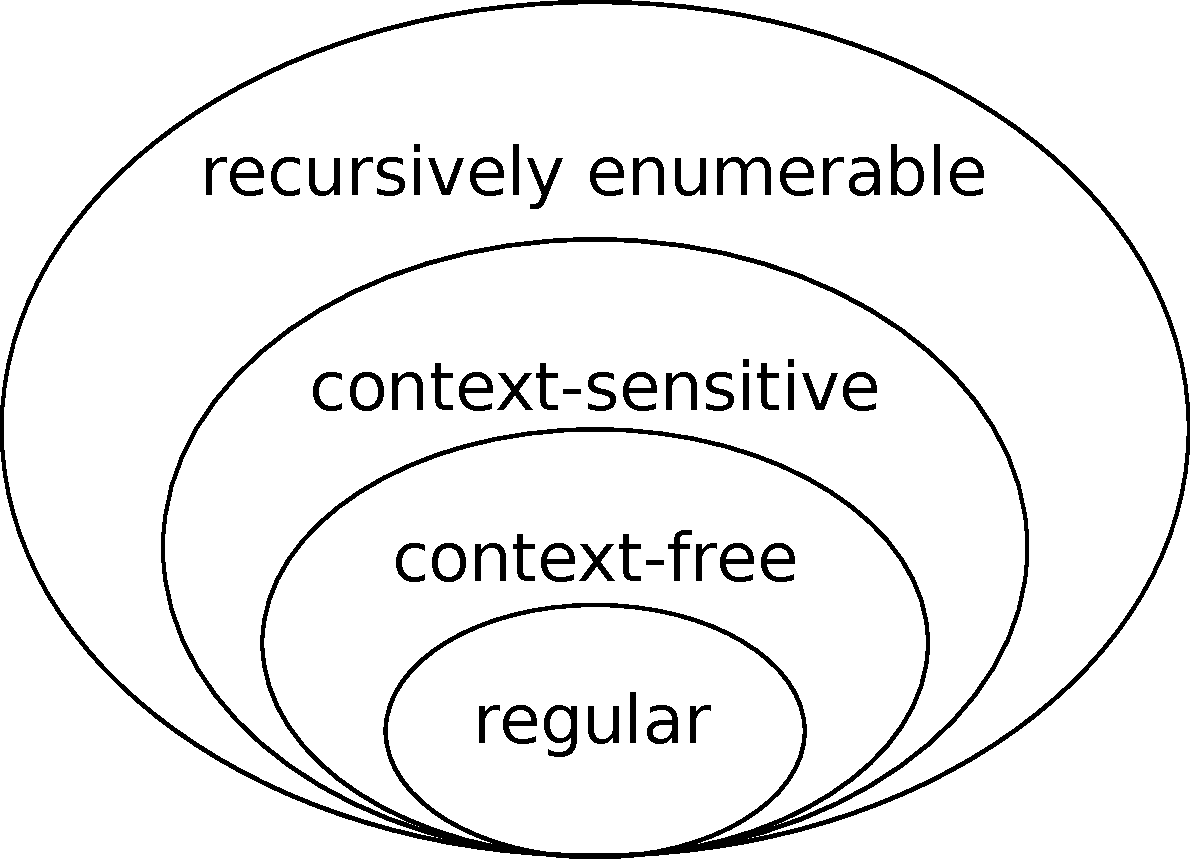
\includegraphics[width=0.6\linewidth]{images/chomsky-hierarchy}
\end{center}

\section{Regular Languages}

\subsection{Closures}
Where $R$ is a regular language, $L$ is `not regular', and $?$ is Unknown.

% Figure out the width of the third coulumn
\settowidth{\templength}{$R \cap R \spto R$}
\addtolength{\templength}{1cm}
\begin{tabular}{lp{\templength}l}
\textbf{Closed:}       &                    & \textbf{Unclosed:} \\
$\overline{R} \spto R$ & $h(R) \spto R$     & $R \cap L \spto ?$ \\
$R^* \spto R$          & $R \cup R \spto R$ & $R \cup L \spto ?$\\
$R^R \spto R$          & $R \cap R \spto R$ & $L \cup L \spto ?$\\
$RR \spto R$           & $R \spbackslash R \spto R$ & \\
\end{tabular}

\subsection{Pumping Lemma}
\begin{align*}
\exists N \in \mathbb{N}: & \\
         \forall w \in L: &\; |w| \geq N \impl \\
\exists xyz \in \Sigma^*: & \quad w = xyz \\
                          & \land |xy| \leq N \\
                          & \land y \neq \varepsilon \\
                          & \land \forall i \geq 0: xy^iz \in L
\end{align*}

\section{Context Free Languages}

\columnbreak
\subsection{Closures}
Where $C$ is a context-free language, $R$ is a regular language, and $?$ is
an Unknown language.

\settowidth{\templength}{$C \cup C \spto C$}
\addtolength{\templength}{1cm}
\begin{tabular}{lp{\templength}l}
\textbf{Closed:} & & \textbf{Unclosed:} \\
$C^R \spto C$ & $C \cup C \spto C$ & $\overline{C} \spto ?$\\
$C^* \spto C$ & $C \cap R \spto C$ & $C \cap C \spto ?$\\
$CC \spto C$  & $C \cup R \spto R$ & $C \spbackslash C \spto ?$\\
$h(C) \spto C$ & & \\
\end{tabular}

\subsection{Pumping Lemma}
\begin{align*}
  \exists N \in \mathbb{N}: & \\
          \forall w \in L : & |w| \geq N \impl \\
\exists uvxyz \in \Sigma^*: & \quad w = uvxyz \\
                            & \land |vy| > 0 \\
                            & \land |vxy| \leq N \\
                            & \land \forall i \geq 0: uv^ixy^iz \in L
\end{align*}

\subsection{Ambiguous Context Free Languages}
These are languages that have two separate parse-trees. To prove
that a language is ambiguous, show that it actually has two separate
parse-trees.

Example ambiguous grammar:
\[
    E \spto E + E \;|\; E * E \;|\; \texttt{NUMBER}
\]

\subsection{Consistency and Completeness}
\begin{description}
    \item[{\small Consistency:}] All strings generated by a grammar are 
    in the language.
    \item[{\small Completeness:}] The grammar generates all strings 
    in the language.
\end{description}

You cannot know that a grammar defines a language until you show both.
For example, if we want to define the language $\{a^nb^n | n \in \mathbb{N}\}$,
the grammar:
\[
    S \spto aabb
\]
Is \textit{consistent} because it only generates strings in the language,
but not complete because it doesn't generate all strings in the language.
Likewise, the grammar:
\[
    S \spto aS \;|\; bS \;|\; \varepsilon 
    \;\;\quad (\textit{grammar for }\{a, b\}^*)
\]
Is complete, it generates all possible strings in the language, but not
consistent because it generates many strings that are, in-fact, outside of
the language.

\subsection{RL and LL Grammar Conversion}


\end{multicols*}
\end{document}
